% CVPR 2022 Paper Template
% based on the CVPR template provided by Ming-Ming Cheng (https://github.com/MCG-NKU/CVPR_Template)
% modified and extended by Stefan Roth (stefan.roth@NOSPAMtu-darmstadt.de)

\documentclass[10pt,twocolumn,letterpaper]{article}

%%%%%%%%% PAPER TYPE  - PLEASE UPDATE FOR FINAL VERSION
%\usepackage[review]{cvpr}      % To produce the REVIEW version
%\usepackage{cvpr}              % To produce the CAMERA-READY version
\usepackage[pagenumbers]{cvpr} % To force page numbers, e.g. for an arXiv version

% Include other packages here, before hyperref.
\usepackage{graphicx}
\usepackage{amsmath}
\usepackage{amssymb}
\usepackage{booktabs}
\usepackage{pgfgantt}
\usepackage{array}
\usepackage{url} 

% It is strongly recommended to use hyperref, especially for the review version.
% hyperref with option pagebackref eases the reviewers' job.
% Please disable hyperref *only* if you encounter grave issues, e.g. with the
% file validation for the camera-ready version.
%
% If you comment hyperref and then uncomment it, you should delete
% ReviewTempalte.aux before re-running LaTeX.
% (Or just hit 'q' on the first LaTeX run, let it finish, and you
%  should be clear).
\usepackage[pagebackref,breaklinks,colorlinks]{hyperref}
\usepackage[bottom]{footmisc}


% Support for easy cross-referencing
\usepackage[capitalize]{cleveref}
\crefname{section}{Sec.}{Secs.}
\Crefname{section}{Section}{Sections}
\Crefname{table}{Table}{Tables}
\crefname{table}{Tab.}{Tabs.}


\def\groupID{Team-Q}
\def\subjectNum{COMP6721}
\def\subName{Applied Artificial Intelligence } 



\begin{document}



\definecolor{barblue}{RGB}{206,34,34}
\definecolor{groupblue}{RGB}{120,34,34}
\definecolor{linkred}{RGB}{165,0,33}
% \renewcommand\sfdefault{phv}
% \renewcommand\mddefault{mc}
% \renewcommand\bfdefault{bc}


%%%%%%%%% TITLE - PLEASE UPDATE
\title{Proposal for \subjectNum-\subName Project - Group Q}

\author{Rohan Chopra\\
\small 40233019\\
\and
Harman Singh Jolly\\
\small 40204947\\
\and
Harman Preet Kaur\\
\small 40198317\\
\and
Abhishek Handa\\
\small 40231719\\
}
\maketitle
%%%%%%%%% BODY TEXT
\section{Problem Statement and Application}
\label{sec:intro}
The destruction caused by COVID-19 has created a need for diagnosis 
that is reliable, effective, and fast. Chest 
X-ray acquisition is easy but needs to be evaluated by an expert 
radiologist. We propose that a deep CNN model can help 
diagnose new diseases much 
faster and accurately, so we plan to create models that will 
classify multiple lung diseases like COVID-19 and 
Atelectasis. This will allow us to reduce the turn-around-times 
for diagnosis of new diseases considerably. 
There are a number of challenges that we foresee, the datasets 
are highly imbalanced so we will have to take corrective measures. Images 
from different X-Ray scanners have different radiographic contrast 
\cite{andrew2022rad} this could have a negative impact on our model's results. 
In some cases, multi-level classification might be required as the patient might 
be affected by multiple diseases.
 
We will try different models to solve this problem and present a 
detailed comparison of the results. After evaluating the results, 
we will choose the best model in terms of both efficiency and 
accuracy. We will try to make use of data augmentation and 
transfer learning to tackle the small dataset problem and design 
our custom CNN which could get us better results 
than the existing architectures. 
%-------------------------------------------------------------------------
\section{Image Dataset Selection}
\label{sec:dataset}
We will use three chest X-Ray datasets with different diseases as listed in \cref*{tab:selDataset} to train and evaluate our models.
\begin{table}
  \centering
  \begin{tabular}{p{1.6cm}|p{3.4cm}|wc{0.8cm}|p{1cm}}
    \toprule
    Dataset & No. of Images & Classes & Image Size\\
    \midrule
    Pneumonia \& COVID-19 \cite{covidchest} & 1,583 (Normal) + 576 (COVID-19) + 4,273 (Pneumonia) = \textbf{6,432} & 3 & Variable\\
    \midrule
    Pneumonia \cite{kermany2018labeled} \cite{kagglepneu} & 1,583 (Normal) + 1,493 (Viral Pneumonia) + 2,780 (Baterial Pneumonia)  = \textbf{5,856} & 3 & 224 x 224\\
    \midrule
    Chest X-Ray8 \cite{wang2017chestx} \cite{kaggle8} & 60,190 (Normal) + 16,610 (Infiltration) + 8,284 (Atelectasis) = \textbf{85,084} & 3 & 1024 x 1024\\
    \bottomrule
  \end{tabular}
  \caption{Shortlisted Datasets.}
  \label{tab:selDataset}
\end{table}
\section{Possible Methodology}
As our datasets are from different sources, we will explore different 
pre-processing techniques like histogram equalization, Gaussian blur 
\cite{gielczyk2022pre}, updating contrast and image flipping in PyTorch 
using functions like normalize, gaussian\_blur and equalize \cite{transforms} 
to make training easier for our CNN. We will explore several neural network architectures like VGG 16 \cite{simonyan2014very}, 
Inception V3 \cite{szegedy2016rethinking}, Resnet \cite{he2016deep}, and produce our own Custom CNN model as well 
with different depth, size of kernel, strides and types of layers. 
To train our models, we will use cross-entropy loss and experiment 
with optimizers \cite{dloptimizers} like Stochastic Gradient Descent, Adam, AdaDelta \cite{kandel2020comparative} etc. 
to select the optimizer that gives us a lower loss with less epochs. 
To ensure that our model does not get stuck at a local minima, we 
will try different learning rate decay methods. While training, we 
will tweak different hyperparameters like epoch, activation functions, 
and batch size to ensure that we get a well performing model. As 
the size of our dataset is small, we plan on experimenting with 
techniques like data augmentation and transfer learning to improve 
our results. To find the best hyperparameters, we will perform ablation 
studies and try to make use of Bayesian hyperparameter optimization 
\cite{balandat2020botorch}. 

Given that our datasets are highly imbalanced, we will not rely on 
accuracy and will explore different metrics like confusion matrix, 
ROC Curve and F-Measure \cite{fmeasure}. We will also consider the FLOPs of our models 
as one of the key metrics. To explain the results of our models, 
we plan on using SHAP \cite{NIPS2017_8a20a862} and GradCAM \cite{jacobgilpytorchcam} which will help us diagnose our 
models and also help end users gain more confidence in our model's decisions.

We plan to make use of the Google Colab platform to train our classifiers. 
In order to seamlessly collaborate and transfer changes from our local 
system to the training system on Colab we will make use of git and Google Drive.
\clearpage
\begin{figure*}[!h]
  \vspace{22.6cm}
  \hspace{2cm}
  \begin{tikzpicture}
    
    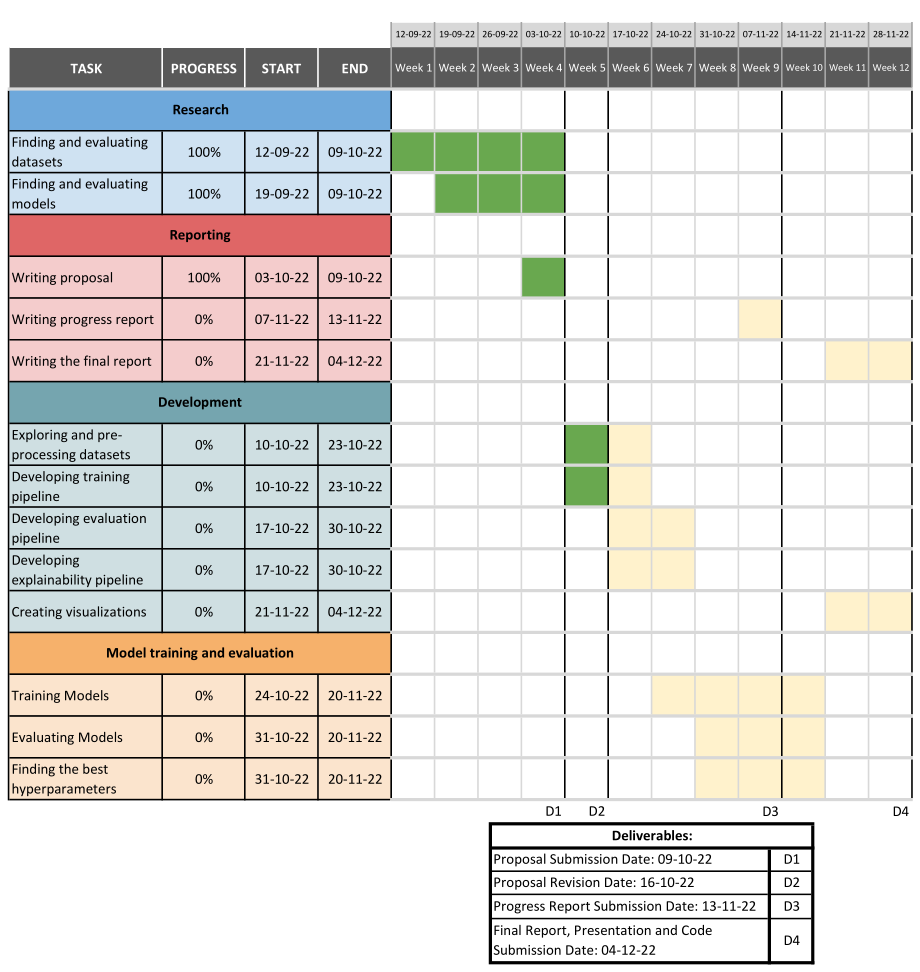
\includegraphics[width=24cm,angle=90]{gantt_chart.png}
\end{tikzpicture}
\caption{Gantt Chart.}
\end{figure*}

\clearpage
%%%%%%%%% REFERENCES
{\small
\bibliographystyle{ieee_fullname}
\bibliography{egbib}
}

\end{document}
